%\documentclass[titlepage]{jsarticle}
%\usepackage{array}
%\usepackage{booktabs}
%\usepackage{amsmath}
%\usepackage[dvipdfmx]{graphicx}
%\usepackage{float}
%\usepackage[version=3]{mhchem}
%\begin{document}

\section{加速器の原理}

本実験では京都大学小型中性子源KUANS(Kyoto University Accelerator-driven Neutron Source)で実験を行った。本節ではこの加速器について説明する。
KUANSの性能は以下のようになっている。
\begin{table}[htb]
  \begin{tabular}{lcrr}
    加速器&陽子線形加速器\\
加速粒子&陽子\\
最大加速エネルギー&3.5MeV\\
最大電流&100 $\mu$ \\
中性子発生ターゲット&Be\\
発生中性子エネルギー&keV~熱中性子(約2000m/s)\\
中性子減速材&ポリエチレン($10\times10\times10$ cm$^3$)\\
  \end{tabular}
\end{table}
\subsection{中性子発生方法}
まず陽子線形加速器によって陽極で発生させた陽子を電圧で加速させ、シールド内に収められているBeターゲットへと衝突させる。
この際起こる以下の反応、\ce{p+^{9}Be->n+^{9}B}
によって中性子を発生させている。
しかし、このままの中性子は速すぎて実験に向かないので、KUANSでは減速材を用いて減速させ、熱中性子とした後に陽子ビームの向きと90$^{\circ}$をなす方向に導いて実験用中性子ビームとして利用している。
\subsection {TOF(Time Of Flight)}
TOFとは一般的に粒子が加速されてから検出器に入るまでに要する時間のことである。(TOFの測定方法については中性子検出器の項で述べる。)
以降、本実験におけるTOFとは陽子線形加速器に電圧が印加されてから発生した中性子が検出器に入るまでに掛かる時間のことを指すこととする。
このTOFは以下のように表せる。

本実験では波長が重要な値となるので、補正したTOFから以下の式によって中性子の波長を算出した。







\subsection 中性子のTOF分布







\subsection Lim 
\begin{figure}
\begin{center}
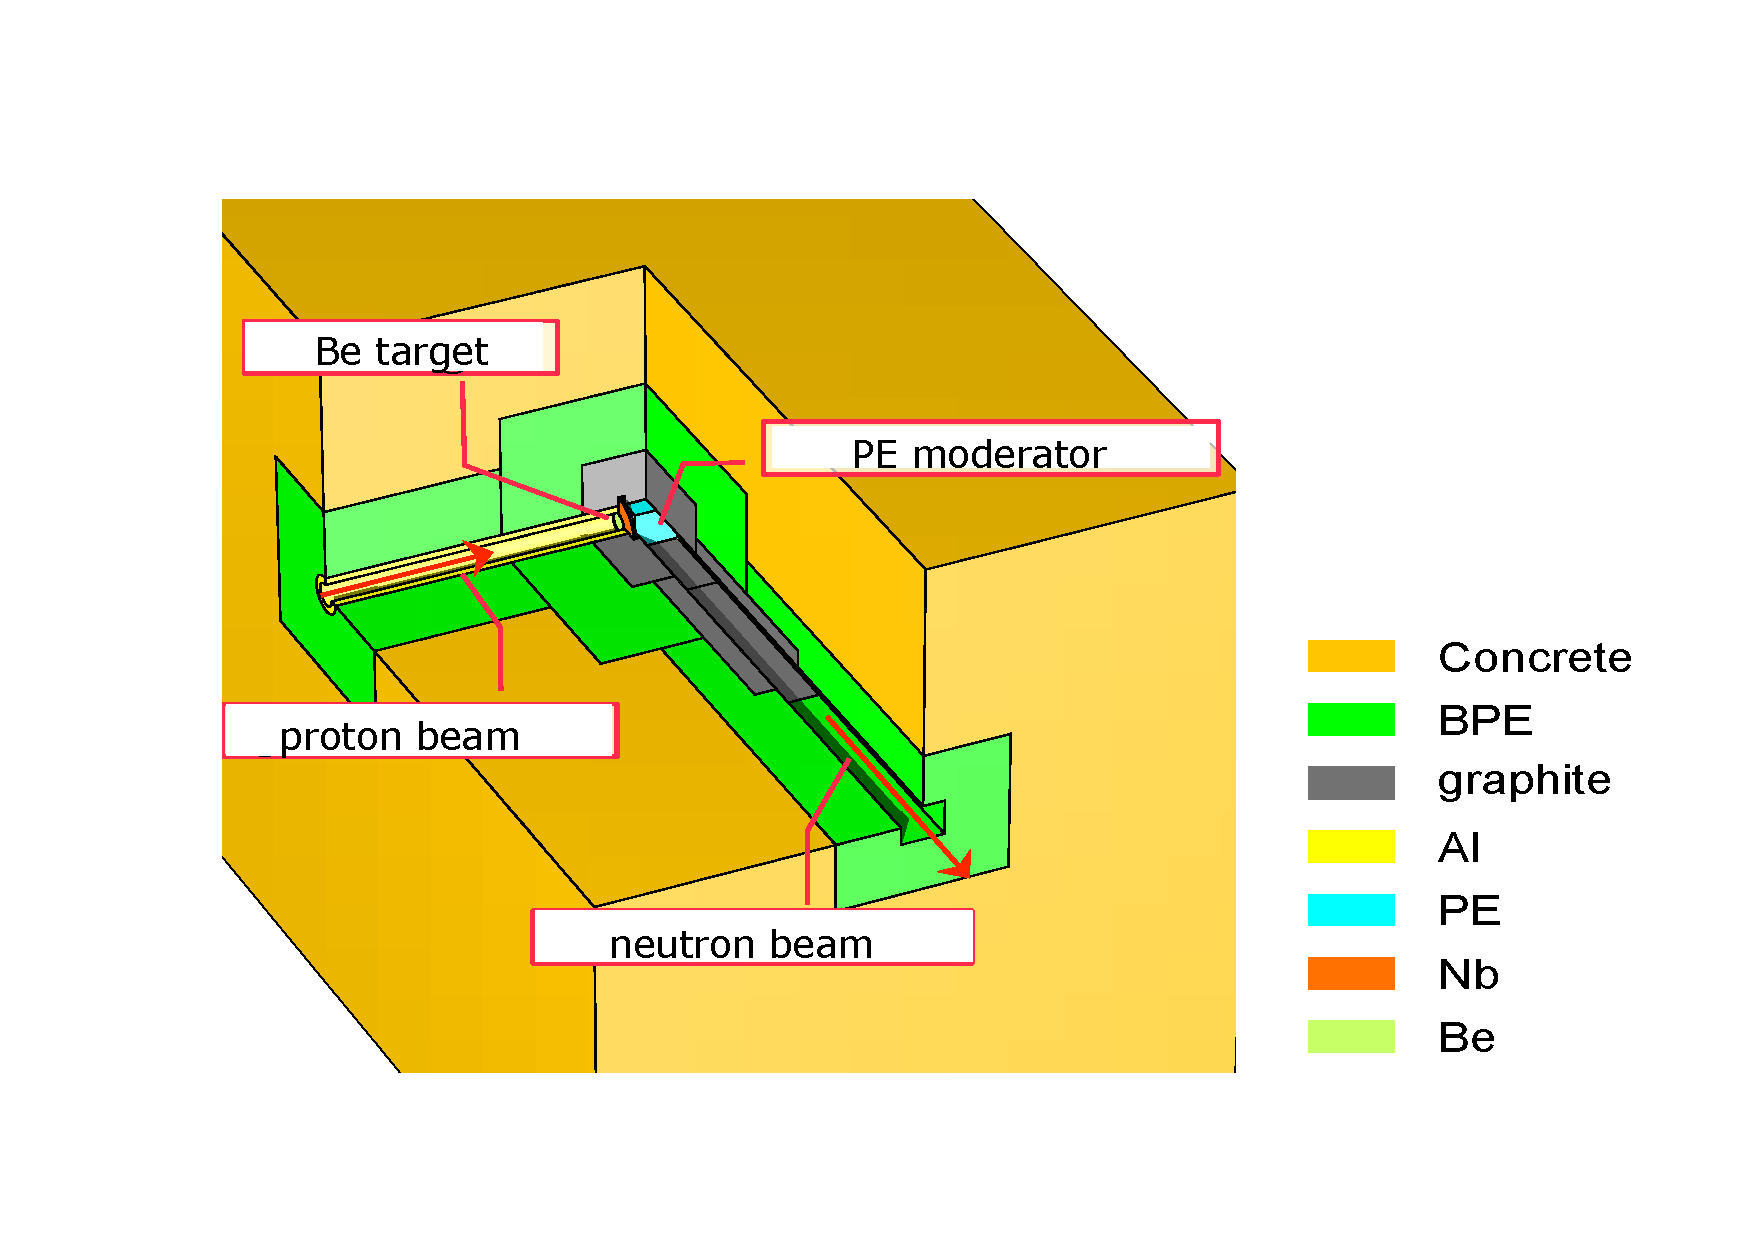
\includegraphics[width=9cm]{accelerator/kuans_inner.pdf}
\caption{KUANSの遮蔽体の内部構造} \label{kuans_inner}
\end{center}
\end{figure}

%\end{document}
